% !TeX root = ../main.tex
\section{Тестовое воздействие и результаты имитационного моделирования}

Для проверки работоспособности разработанного тракта цифровой обработки было сформировано тестовое воздействие в виде радиоимпульса с линейной частотной модуляцией (ЛЧМ) на фоне аддитивного белого гауссова шума. После выполнения этапов цифровой демодуляции (перемножения с цифровым гетеродином) и фильтрации нижних частот, спектр сигнала переносится в область нулевой частоты. 

На рисунке \ref{fig:envelope} показана сформированная комплексная огибающая сигнала на выходе тракта предварительной обработки. 

\begin{figure}[H]
    \centering
    % Если переименуешь файл, поменяй image_c5bdbf.png на свое название
    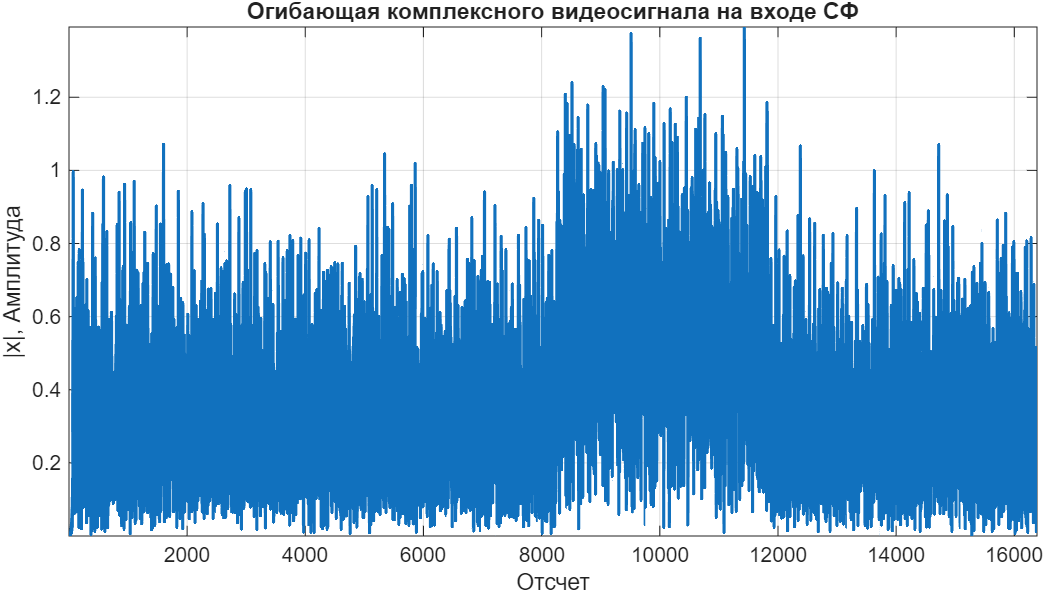
\includegraphics[width=0.85\textwidth]{image_c5bdbf.png} 
    \caption{Огибающая комплексного видеосигнала на входе согласованного фильтра}
    \label{fig:envelope}
\end{figure}

Как видно из графика, сформированный видеоимпульс сохраняет прямоугольную огибающую, а высокочастотные продукты гетеродинирования эффективно подавлены.

Окончательная внутриимпульсная обработка производится в согласованном фильтре. Для детального анализа структуры боковых лепестков на рисунке \ref{fig:zoom} представлен увеличенный фрагмент отклика фильтра (сжатый импульс), вычисленного методом сегментированной свертки \texttt{fftfilt}.

\begin{figure}[H]
    \centering
    % Если переименуешь файл, поменяй image_c5bda3.png на свое название
    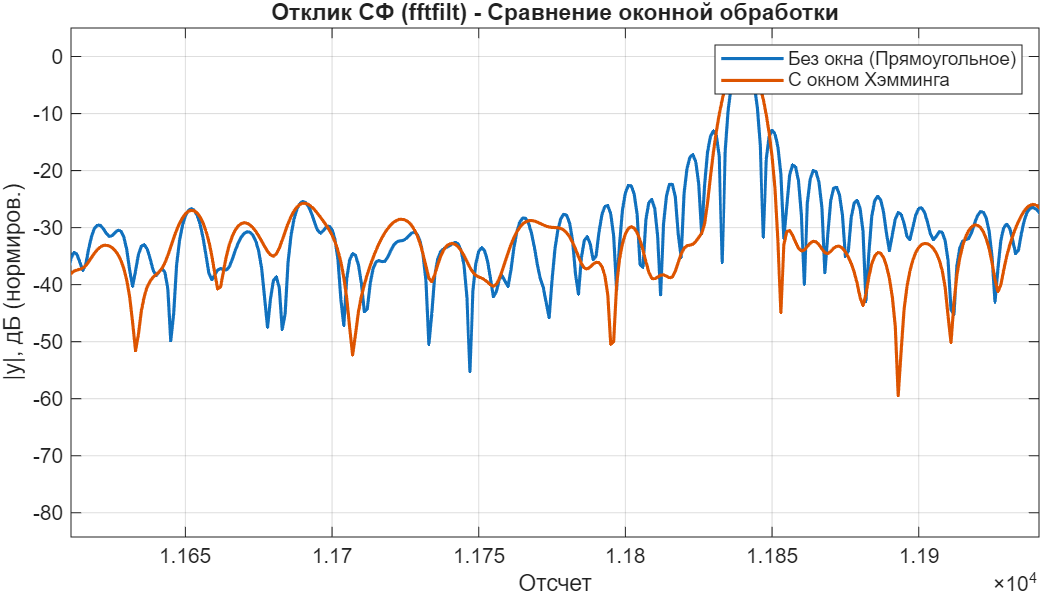
\includegraphics[width=0.85\textwidth]{image_c5bda3.png} 
    \caption{Отклик СФ (fftfilt) крупным планом: сравнение оконной обработки}
    \label{fig:zoom}
\end{figure}

Сравнение двух методов весовой обработки наглядно демонстрирует, что без использования окна уровень первого бокового лепестка составляет около $-13.3$~дБ относительно главного пика. Применение весового окна Хэмминга к опорному сигналу позволяет существенно снизить уровень ближних боковых лепестков до $-42.8$~дБ, что предотвращает маскирование слабых эхо-сигналов. При этом наблюдается закономерное расширение главного лепестка по уровню $-3$~дБ примерно в $1.35 \dots 1.4$ раза.

В качестве дополнительного исследования была проведена проверка математической тождественности различных алгоритмов вычисления согласованной фильтрации: прямой временной свертки (FIR), спектрального метода через БПФ/ОБПФ и сегментированной быстрой свертки с перекрытием (\texttt{fftfilt}). Результаты совмещения нормированных откликов представлены на рисунке \ref{fig:compare}.

\begin{figure}[H]
    \centering
    % Если переименуешь файл, поменяй image_c5bd9b.png на свое название
    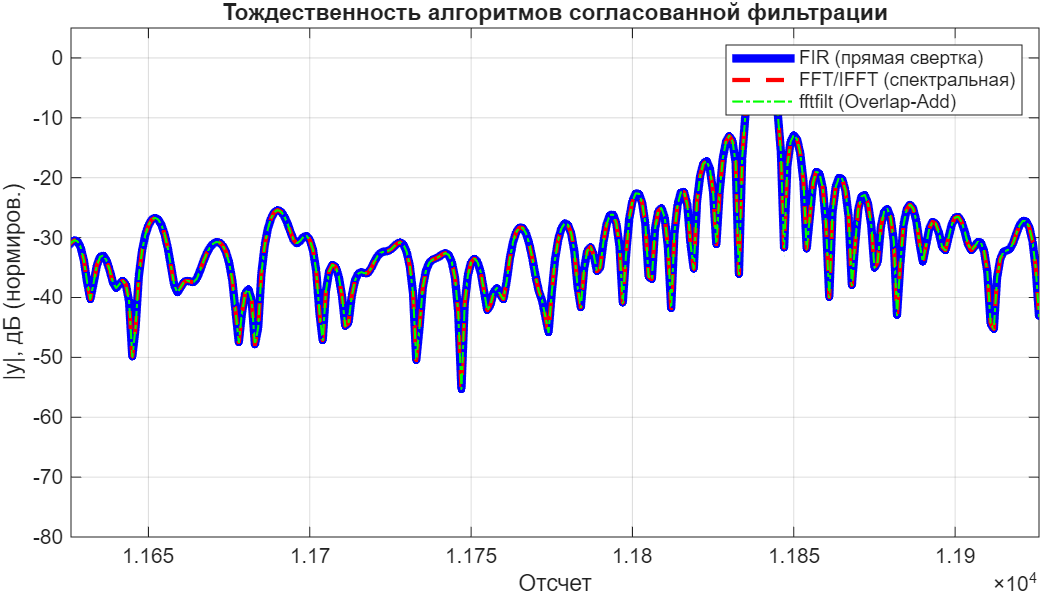
\includegraphics[width=0.85\textwidth]{image_c5bd9b.png} 
    \caption{Тождественность алгоритмов согласованной фильтрации}
    \label{fig:compare}
\end{figure}

Графики откликов всех трех методов полностью совпадают на всех участках временной шкалы. Это подтверждает, что блочный метод сегментированной свертки работает абсолютно корректно и не вносит искажений, являясь при этом наиболее вычислительно эффективным для обработки длинных потоков данных.